\section{Exponential Distribution}
\label{sec:expon-distr}
As we will see in the sections to come, the modeling and analysis of
any queueing system involves the specification of the (probability)
distribution of the time between consecutive arrival epochs of jobs,
or the specification of the distribution of the number of jobs that
arrive in a certain interval.  For the first case, the most common
distribution is the exponential distribution, while for the second it
is the Poisson distribution.  For these reasons we start our
discussion of the analysis of queueing system with these two
exceedingly important distributions. In the ensuing sections we will
use these distributions time and again.

As mentioned, one of the most useful models for the inter-arrival
times of jobs assumes that the sequence $\{X_i\}$ of inter-arrival
times is a set of \recall{independent and identically distributed
  (i.i.d.)}  random variables.  Let us write $X$ for the generic
random time between two successive arrivals. For many queueing
systems, measurements of the inter-arrival times between consecutive
arrivals show that it is reasonable to model an inter-arrival $X$ as
an \recall{exponentially distributed} random variable, i.e.,
\begin{equation*}
  \P{X \leq t} = 1- e^{-\lambda t} := G(t)
\end{equation*}
The constant $\lambda$ is often called the \recall{rate}. The reason
behind this will be clarified once we relate the exponential
distribution to the Poisson process in
Section~\ref{sec:poisson-distribution}.  In the sequel we often write $X\sim \exp{\lambda}$ to mean that $X$ is exponentially distributed with rate $\lambda$. 


Let us show with simulation how the exponential distribution
originates. Consider $N$ people that regularly visit a shop. We assume
that we can characterize the interarrival times
$\{X_k^i, k=1,2, \ldots\}$ of customer $i$ by some distribution
function, for instance the uniform distribution. Then,
\begin{equation*}
A_k^i = A_{k-1}^i + X_k^i = \sum_{j=1}^n X_j^i,
\end{equation*}
is the arrival moment of the $k$th visit of customer $i$.  Now the
show owner `sees' the superposition of the arrivals of the
customers. One way to compute the arrival moments of all customers is
to put all the numbers $\{A_k^i, k=1,\ldots,n, i=1,\ldots,N\}$ into
one set, and sort these numbers in increasing order. This results in
the (sorted) set of arrivals $\{A_k, k=1,2,\ldots\}$ at the shop, and
then
\begin{equation*}
X_k = A_k - A_{k-1}
\end{equation*}
must be the inter-arrival time between the $k-1$th and $k$th visit to
the shop.  Thus, starting from interarrival times of individual
customers we constructed interarrival times as seen by the shop. 

To plot the \recall{empirical distribution function}, or the histogram,
of the inter-arrival times at the shop, consider
\begin{equation*}
  \PP{n}{X \leq x} = \frac1n\sum_{i=1}^n \1{X_i\leq x},
\end{equation*}
where\footnote{More generally, $\1{A}$ is the indicator function of
  the event $A$ meaning that $\1{A}=1$ if $A$ is true and $\1{A}=0$
  otherwise.} $\1{X_i\leq x}=1$ if $X_i\leq x$ and $\1{X_i\leq x}=0$
if $X_i> x$.  Thus, for a simulation of duration $n$, this formula
counts all interarrival times that are smaller than $x$.  

We now compare $\mathbb{P}_n$ to the density of the exponential
distribution, i.e., to $\lambda e^{-\lambda t}$ several simulation
scenarios.  As a first example, take $N=1$ and let the computer
generate $n=100$ uniformly distributed numbers on the set $[4,
6]$.
Thus, the time between two visits of an individual customer is
somewhere between $4$ and $6$ hours. In a second simulation we take
$N=3$, and in the third, $N=10$. The emperical distributions are
shown, from left to right, in the three panels in
Figure~\ref{fig:uniform}. The continuous curve is the graph of
$\lambda e^{-\lambda x}$ where $\lambda = N/5$.  Recall from
Eq.~(\ref{eq:54}) that when $N$ persons visits the shop, each with an
average interarrival time of $5$ hours, it must be that the arrival
rate is $N/5$. As a second example we take the inter-arrival times to
be normally distributed times with mean $5$ and $\sigma=1$. The
results are shown in the second row of Figure~\ref{fig:uniform}.

\begin{figure}[ht]
  \centering
  \begin{tabular}[h]{c}
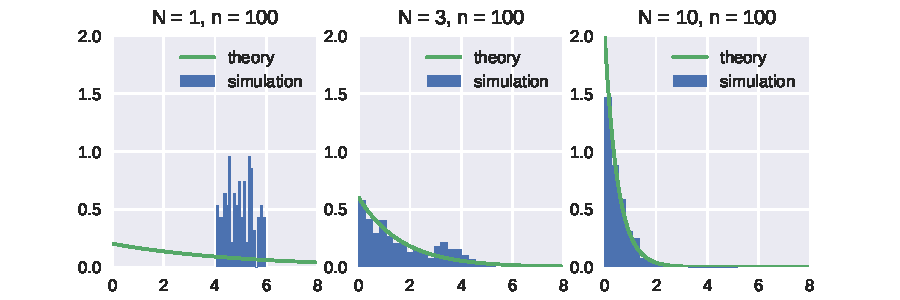
\includegraphics{uniform_N_10_n_100} \\
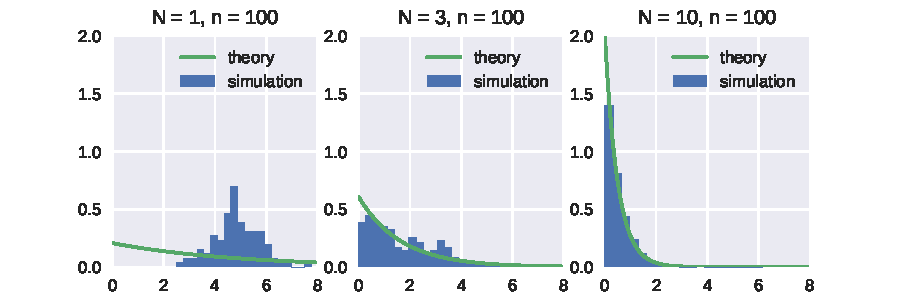
\includegraphics{normal_N_10_n_100}
  \end{tabular}
  \caption{The interarrival process as seen by the shop owner. Observe
    that the green line intersects the $y$-axis at level $N/5$, which
    is equal to the arrival rate when $N$ persons visit the shop. The
    parameter $L$ is the simulation length, i.e., the number of
    arrivals per customer.}
  \label{fig:uniform}
\end{figure}

As the graphs show, even when the customer population consists of 10
members each visiting the shop with an inter-arrival time that is
quite `far' from exponential, the distribution of the inter-arrival
times as observed by the shop is very well approximated by an
exponential distribution. Thus, for a real shop, with many thousands
of customers, or a hospital, call center, in fact for nearly every
system that deals with random demand, it seems reasonable to use the
exponential distribution to model inter-arrival times.  In conclusion,
the main conditions to use an exponential distribution are: 1)
arrivals have to be drawn from a large population, and 2) each of the
arriving customers decides, independent of the others, to visit the
system.

Another reason to use the exponential distribution is that an
exponentially distributed random variable is \recall{memoryless},
that is, $X$ is memoryless if it satisfies the property that
\begin{equation*}
  \P{X > t+h | X>t} = \P{X>h}.
\end{equation*}
In words, the probability that $X$ is larger than some time $t+h$,
conditional on it being larger than a time~$t$, is equal to the
probability that $X$ is larger than $h$. Thus, no matter how long we
have been waiting for the next arrival to occur, the time that it
occurs in the next $h$ seconds remains the same.  This property seems
to be vindicated also in practice: suppose that a patient with a
broken arm just arrived at the emergency room of a hospital, what does
that tell us about the time the next patient will be brought in? Not
much, as most of us will agree.

It can be shown that only exponential random variables have the
memoryless property. The proof of this fact requires quite some work;
we refer the reader to the literature if s/he want to check this.

Finally, the reader should realize that it is simple, by means of
computers, to generate exponentially distributed inter-arrival
times. Thus, it is easy to use such exponentially distributed random
variables to simulate queueing systems. 



\begin{question}(Conditional probability)

  We have to give one present to one of three children. As we cannot
  divide the present into parts, we decide to let `fate decide'. That
  is, we choose a random number in the set $\{1, 2, 3\}$. The first
  child that guesses the number wins the present. Show that the
  probability of winning the present is the same for each child.
\hint{For the second child, condition on the event that the first does not chose the right number.}
\begin{solution}
    Use the definition of conditional probability
    ($\P{A|B} = \P{AB}/\P{B}$, provided $\P{B}>0$)

    The probability that the first child to guess also wins is
    $1/3$. What is the probability for child number two? Well, for
    him/her to win, it is necessary that child one does not win and
    that child two guesses the right number of the remaining
    numbers. Assume, without loss of generality that child 1 chooses
    $3$ and that this is not the right number. Then 
    \begin{equation*}
      \begin{split}
&\P{\text{Child  2 wins}} \\
&= \P{\text{Child 2 guesses the right number and child 1 does not win}} \\
&= \P{\text{Child 2 guesses the right number} \given \text{ child 1 does not win}}
\cdot \P{\text{Child 1 does not win}} \\
&= \P{\text{Child 2 makes the right guess in the set $\{1,2\}$}}\cdot \frac 23 \\
&= \frac 1 2\cdot \frac 23  = \frac 1 3.
      \end{split}
    \end{equation*}
    Similar conditional reasoning gives that child 3 wins with probability $1/3$. 
  \end{solution}
\end{question}

\begin{question}
  Assume that the time $X$ to fail of a machine is uniformly
  distributed on the interval $[0,10]$. If the machine fails at time
  $t$, the cost to repair it is $h(t)$. What is the expected repair
  cost? 
  \begin{solution}
    Write for $F(x) = \P{X\leq x}$ and $f(x) = \d F(x)/\d x$ for the
    density of $F$.
    \begin{equation*}
      \begin{split}
\E{h(X)}
&= \int_0^{10} \E{h(X) \given X = x} \P{X\in \d x} \\
&= \int_0^{10} \E{h(x) \given X = x} \d F(x) \\
&= \int_0^{10} \E{h(x) \given X = x} F(\d x) \\
&= \int_0^{10} \E{h(x) \given X = x} f(x) \d x \\
&= \int_0^{10} h(x)\frac{\d x}{10}.
      \end{split}
    \end{equation*}
    Here we introduce some notation that is commonly used in the
    probabity literature to indicate the same conceptual idea, i.e,
    $\P{X\in \d x} = \d F(x) = F(\d x) = f(x) \d x$, where the last
    equality follows from the fact that $F$ has a density $f$
    everywhere on $[0,10]$. 

    The concept of conditional expectation is of fundamental
    importance in probability theory. Any \emph{good} probability book
    defines this concept as a random variable measurable with respect
    to some $\sigma$-algebra. In this course we will not deal with
    this elegant idea, due to lack of time. 

  \end{solution}
\end{question}


\begin{question}
  Show that an exponentially distributed random variable is
  memoryless.  
   \hint{Condition on the event ${X>t}$. }
  \begin{solution}
This is easy, but be sure you can do it. 

To see that an exponentially
distributed is memoryless, use the definition of conditional
probability ($\P{A|B} = \P{AB}/\P{B}$, provided $\P{B}>0$):
\begin{equation*}
  \P{X>t+h|X>t} = \frac{\P{X>t+h, X>t}}{\P{X>t}} = \frac{\P{X>t+h}}{\P{X>t}} = \frac{e^{-\lambda(t+h)}}{e^{-\lambda t}} = e^{-\lambda h} = \P{X>h}.
\end{equation*}
  \end{solution}
\end{question}

\begin{question} 
  If the random variable $X\sim\exp(\lambda)$, show that
 \begin{equation*}
    \E X = \int_0^\infty t \,\d F(t) = \int_0^\infty t f(t)\, \d t =
    \int_0^\infty t \lambda e^{-\lambda t}\, \d t = \frac{1}\lambda,
  \end{equation*}
  where~$f$ is the density function of the distribution function $F$ of $X$.
  \begin{solution}
    \begin{equation*}
      \begin{split}
\E{X} 
&= \int_0^\infty \E{X\given X=t} f(t) \d t \\
&= \int_0^\infty t \lambda e^{-\lambda t} \d t, \quad\text{density is } \lambda e^{-\lambda t} \\
&=   \lambda^{-1} \int_0^\infty u e^{-u}\, \d u, \quad \text{ by  change of variable $u=\lambda t$},   \\
&=  -\lambda^{-1}\left. t e^{- t}\right|_0^\infty + \lambda^{-1} \int_0^\infty e^{- t} \d t\\
&=  - \lambda^{-1} \left. e^{- t} \right|_0^\infty =  \frac1\lambda.
      \end{split}
    \end{equation*}
  \end{solution}
\end{question}

\begin{question} 
  If the random variable $X\sim\exp(\lambda)$, show that
  \begin{equation*}
  \E{X^2}= \int_0^\infty t^2 \lambda e^{-\lambda t}\, \d t =  \frac{2}{\lambda^2}.
  \end{equation*}
  \begin{solution}
    \begin{equation*}
      \begin{split}
\E{X^2} 
&= \int_0^\infty \E{X^2\given X=t} f(t) \d t \\
&= \int_0^\infty t^2 \lambda e^{-\lambda t} \d t \\
&=   \lambda^{-2} \int_0^\infty u^2 e^{-u}\, \d u, \quad \text{ by  change of variable $u=\lambda t$},   \\
&= -\lambda^{-2}\left. t^2 e^{- t}\right|_0^\infty + 2\lambda^{-2}\int_0^\infty t e^{- t} \d t \\
&=  -2\lambda^{-2}\left. t e^{- t}\right|_0^\infty + 2\lambda^{-2} \int_0^\infty e^{- t} \d t\\
&=  - 2\lambda^{-2} \left. e^{- t} \right|_0^\infty \\
&=  2/\lambda^2.
      \end{split}
    \end{equation*}
  \end{solution}
\end{question}

\begin{question} 
  If the random variable $X\sim\exp(\lambda)$, show that the \recall{variance}
  \begin{equation*}
  \V X = \E X^2 - (\E X)^2 = \frac{1}{\lambda^2}.
  \end{equation*}
  Recall in particular this middle term to compute $\V X$; it is very
  practical.
  \begin{solution}
    By the previous problems, $\E{X^2}=2/\lambda^2$ and $\E X = \lambda$. 
  \end{solution}
\end{question}

\begin{question}
 Define the \recall{square coefficient of variation (SCV)} as
  \begin{equation}
C_a^2 = \frac{\V X}{(\E X)^2}.
  \end{equation}
  Prove that when $X$ is exponentially distributed, $C_a^2 =1$.  As
  will become clear later, the SCV is a very important concept in
  queueing theory. Memorize it as a measure of \emph{relative
  variability}.
\begin{solution}
  By the previous problems, $\V X = 1/\lambda^2$ and $\E X=1/\lambda$.
\end{solution}
\end{question}

\begin{question}\label{ex:33}
 If $X$ is an exponentially distributed random variable with
    parameter $\lambda$, show that its moment generating function
    \begin{equation*}
    M_X(t) = \E{e^{tX}} = \frac{\lambda}{\lambda-t}.
    \end{equation*}
    \begin{solution}
    \begin{equation*}
      \begin{split}
      M_X(t) &= \E{\exp(t X)} = \int_0^\infty e^{tx} \,\d F(x) 
=\int_0^\infty e^{tx} f(x) \,\d x 
=\int_0^\infty e^{tx} \lambda e^{-\lambda x} \,\d x  \\
&=\lambda \int_0^\infty e^{(t-\lambda)x} \,\d x 
=\frac{\lambda}{\lambda -t}.
      \end{split}
    \end{equation*}
    \end{solution}
  \end{question}

  \begin{question}
 Let $A_i$ be the arrival time of customer $i$ and set $A_0=0$.
    Assume that the inter-arrival times $\{X_i\}$ are i.i.d.  with
    exponential distribution with mean $1/\lambda$ for some
    $\lambda>0$.  Prove that the density of
    $A_i=X_1+X_2+\cdots+X_i=\sum_{k=1}^i X_k$ with $i\geq 1$ is
\begin{equation*}
f_{A_i}(t) = \lambda e^{-\lambda t} \frac{(\lambda t)^{i-1}}{(i-1)!}. 
\end{equation*}
 \hint{ Check the result for $i=1$ by filling in $i=1$ (just to be
     sure that you have read the formula right), and compare the result
     to the exponential density. Then write $A_i =\sum_{i=1}^k X_k$, and compute the moment
     generating function for $A_i$ and use that the inter-arrival times
     $X_i$ are independent. Use the moment generating function  of $X_i$.}
\begin{solution}
 One way to find the distribution of $A_i$ is by using the
    moment generating function $M_{A_i}(t) = \E{e^{t A_i}}$ of
    $A_i$. Let $X_i$ be the inter-arrival time between customers $i$
    and $i-1$, and $M_X(t)$ the associated moment generating
    function. Using the i.i.d. property of the $\{X_i\}$,
\begin{equation*}
  \begin{split}
  M_{A_i}(t) &= \E{e^{t A_i}} = \E{\exp\left(t\sum_{j=1}^{i} X_j\right)} \\
& = \prod_{j=1}^{i} \E{e^{tX_j}} = 
\prod_{j=1}^{i} M_{X_j}(t) = 
\prod_{j=1}^{i} \frac{\lambda}{\lambda -t }
 = \left(\frac{\lambda}{\lambda -t }\right)^i.
  \end{split}
\end{equation*}
From a table of moment generation functions it follows immediately that
$A_i \sim \Gamma(n,\lambda)$, i.e., $A_i$ is Gamma distributed.
\end{solution}

\end{question}

  \begin{question}
    Assume that the inter-arrival times $\{X_i\}$ are i.i.d. and
    $X_i\sim\exp(\lambda)$. Let
    $A_i=X_1+X_2+\cdots+X_i=\sum_{k=1}^i X_k$ with $i\geq 1$. Use the
    density of $A_i$ or the moment generating function of $A_i$ to
    show that
 \begin{equation*}
\E{A_i} = \frac i\lambda,
 \end{equation*}
 that is, the expected time to see $i$ jobs is $i/\lambda$.
  \hint{Use that
    $\int_0^\infty (\lambda t)^i e^{- \lambda t} \d t =
    \frac{i!}\lambda$.
    Another way would be to use that, once you have the moment
    generating function of some random variable $X$,
    $\E X = \frac{\d}{\d t} M(t) |_{t=0}$. }
  \begin{solution}
  \begin{equation*}
\E{A_i} = \int_0^\infty t \P{A_i \in \d t} = \int_0^\infty t f_{A_i} (t) \, \d t  = 
\int_0^\infty t  \lambda e^{-\lambda t} \frac{(\lambda t)^{i-1}}{(i-1)!}\, \d t.
  \end{equation*}
Thus, 
  \begin{equation*}
\E{A_i} = \frac{1}{(i-1)!} \int_0^\infty   e^{-\lambda t} (\lambda t)^i\,\d t = \frac{i!}{(i-1)!\lambda}=\frac{i}\lambda,
  \end{equation*}
  where we used the hint.

What if we would use the moment generating function? 
\begin{equation*}
  \begin{split}
    \E{X} 
&= \left.\frac{\d}{\d t} M(t)\right|_{t=0} \\
&= \left.\frac{\d}{\d t} \left(\frac{\lambda}{\lambda-t}\right)^i\right|_{t=0} \\
&= i \left.\left(\frac{\lambda}{\lambda-t}\right)^{i-1}\frac{\lambda}{(\lambda-t)^2}\right|_{t=0} \\
&= \frac i\lambda \left.\left(\frac{\lambda}{\lambda-t}\right)^{i+1}\right|_{t=0} \\
&= \frac i\lambda.
  \end{split}
\end{equation*}

Of course, $\E A_i = \E{\sum_{k=1}^i X_k} = i \E{X} = 1/\lambda$. 
  \end{solution}
\end{question}


\begin{question}\label{ex:10}
  If $X\sim\exp(\lambda)$ and $Y\sim\exp(\mu)$ and $X$ and $Y$ are
  independent, show that 
  \begin{equation*}
Z=\min\{X,Y\}\sim\exp(\lambda+\mu),
  \end{equation*}
hence $\E Z = (\lambda+\mu)^{-1}$.
  \begin{solution}
    \begin{equation*}
      \begin{split}
      \P{Z>x} 
&= \P{\min{X,Y}>x} = \P{X>x\text{ and } Y>x} = \P{X>x}\P{Y>x} \\
&= e^{-\lambda x} e^{-\mu x} = e^{-(\lambda+\mu)x}.
      \end{split}
    \end{equation*}
  \end{solution}

\end{question}

\begin{question}
  A machine serves two types of jobs. The processing time of jobs of
  type $i$, $i=1,2$, is exponentially distributed with parameter
  $\mu_i$. The type $T$ of job is random and independent of anything
  else, and such that $\P{T=1} = p = 1-q = 1-\P{T=2}$. (An example
  is a desk serving men and women, both requiring different average
  service times, and $p$ is the probability that the customer in
  service is a man.) What is the expected processing time and what is the variance? 
  \begin{solution}
    Let $X$ be the processing (or service) time at the server, and
    $X_i$ the service time of a type $i$ job. Then, 
    \begin{equation*}
      X = \1{T=1} X_1 + \1{T=2} X_2,
    \end{equation*}
    where $\1{}$ is the indicator function, that is, $\1{A}=1$ if the
    event $A$ is true, and $\1{A}=0$ if $A$ is not true. With this,
\begin{equation*}
  \begin{split}
  \E X 
&= \E{\1{T=1} X_1} + \E{\1{T=2} X_2} \\
&= \E{\1{T=1}} \E{ X_1} + \E{\1{T=2}} \E{X_2}, \text{ by the independence of $T$}, \\
&= \P{T=1} /\mu_1 + \P{T=2}/ \mu_2 \\
&= p /\mu_1 + q/ \mu_2 \\
&= p \E{X_1}  + q \E{X_2}.
  \end{split}
\end{equation*}
(The next derivation may seem a bit long, but the algebra is
standard. I include all steps so that you don't have to use pen and
paper yourself if you want to check the result.) Next, using that
\begin{equation*}
\1{T=1}\1{T=2} = 0 \text{ and } \1{T=1}^2 = \1{T=1},
\end{equation*}
we get
\begin{equation*}
  \begin{split}
  \V X 
&= \E{X^2} - (\E X)^2 \\
&= \E{\left(\1{T=1} X_1 + \1{T=2} X_2\right)^2} - \left(\frac{p}{\mu_1}+\frac{q}{\mu_2}\right)^2 \\
&= \E{\1{T=1} X_1^2 + \1{T=2} X_2^2} - \left(\frac{p}{\mu_1}+\frac{q}{\mu_2}\right)^2 \\ 
&= p \E{X_1^2} + q \E{X_2^2} - \left(\frac{p}{\mu_1}+\frac{q}{\mu_2}\right)^2 \\ 
&= p \V{X_1} + p (\E{X_1})^2 + q \V{X_2} + q(\E{ X_2})^2 - \left(\frac{p}{\mu_1}+\frac{q}{\mu_2}\right)^2 \\ 
&= p \V{X_1} + \frac{p}{\mu_1^2} + q \V{X_2} + \frac{q}{\mu_2^2} - \left(\frac{p}{\mu_1}+\frac{q}{\mu_2}\right)^2 \\ 
&= p \V{X_1} + q \V{X_2}
+ \frac{p}{\mu_1^2} + \frac{q}{\mu_2^2}
- \frac{p^2}{\mu_1^2}-\frac{q^2}{\mu_2^2}  -\frac{2pq}{\mu_1\mu_2}\\ 
&= p \V{X_1} + q \V{X_2}
+ \frac{p(1-p)}{\mu_1^2} + \frac{q(1-q)}{\mu_2^2}
-\frac{2pq}{\mu_1\mu_2}\\ 
&= p \V{X_1} + q \V{X_2}
+ \frac{pq}{\mu_1^2} + \frac{qp}{\mu_2^2}
-\frac{2pq}{\mu_1\mu_2}\\ 
&= p \V{X_1} + q \V{X_2}
+ pq(\E{X_1} - \E{X_2})^2.
\end{split}
\end{equation*}

Interestingly, we see that even if $\V X_1 = \V X_2 = 0$, $\V X > 0$
if $\E{X_1} \neq \E{X_2}$. Bear this in mind; we will use these ideas
later when we discuss the effects of failures on the variance of
service times of jobs.

\end{solution}
\end{question}

\begin{question}
  Try to make Figure~\ref{fig:uniform} with simulation.
  \begin{solution}
    I used python to do the simulations. I include the code for you to
    study if you are interested, but you are free to skip it; it is
    not part of the core of the course. 

<<wrap=False, fig=False>>=
import numpy as np
import matplotlib.pyplot as plt
import seaborn as sns
sns.set_context("paper")

np.random.seed(3)


def superposition(a):
    A = np.cumsum(a, axis=1)
    A = np.sort(A.flatten())
    a = A[1:] - A[:-1]
    return a


n = 100 # simulation run length
x = np.arange(0, 8, 0.1)


def makePlot(A, N):
    plt.axis([0, 8, 0, 2])

    X = superposition(A)
    labda = N / A.mean()
    plt.hist(X, 20, normed=1, label='simulation')
    plt.plot(x, labda * np.exp(-labda * x), label="theory")
    plt.title("N = {}, n = {}".format(N, n))
    plt.legend()


plt.figure(figsize=(6, 2))
plt.subplot(131)
N = 1
A = np.random.uniform(4, 6, (N, n))
makePlot(A, N)

plt.subplot(132)
N = 3
A = np.random.uniform(4, 6, (N, n))
makePlot(A, N)

plt.subplot(133)
N = 10
A = np.random.uniform(4, 6, (N, n))
makePlot(A, N)

filename = "figures/uniform_N_{}_n_{}.pdf".format(N, n)
plt.savefig(filename)
plt.close()

# normal distribution

plt.figure(figsize=(6, 2))
plt.subplot(131)
N = 1
A = np.random.normal(5, 1, (N, n))
makePlot(A, N)

plt.subplot(132)
N = 3
A = np.random.normal(5, 1, (N, n))
makePlot(A, N)

plt.subplot(133)
N = 10
A = np.random.normal(5, 1, (N, n))
makePlot(A, N)

filename = "figures/normal_N_{}_n_{}.pdf".format(N, n)
plt.savefig(filename)
plt.close()
@

\end{solution}
\end{question}
  


%%% Local Variables:
%%% mode: latex
%%% TeX-master: "book"
%%% End:
